\chapter{弹性力学伽辽金无网格法}
\section{伽辽金无网格离散}
不失为一般性,弹性力学问题的基本未知量为位移向量$\pmb{u}=\{u_i\},i=1,\dotsb,n_{sd}$,其静力平衡方程为:
\begin{equation}\label{elasticity problems}
\begin{split}
    \sigma_{ij,j}+b_i=0&\text{in}\;\Omega\\
    \sigma_{ij}n_j=t_i&\text{on}\;\Gamma^t\\
    u_i=g_i&\text{on}\;\Gamma^g
\end{split}
\end{equation}
其中$\pmb \sigma=[\sigma_{ij}]$为柯西应力,$\pmb{b}=\{b_i\}$为体力,$\Gamma^t \text{、}\Gamma^g$分别表示为自然和强制边界条件,$\Gamma^t\cup \Gamma^g=\Gamma,\Gamma^t\cap \Gamma^g=\varnothing$,$\pmb{t}=\{t_i\}$和$\pmb{g}=\{g_i\}$分别为自然边界和强制边界上给定的面力和位移,$\pmb{n}=\{n_i\}$是$\Gamma^{t}$的外法线方向。\par
考虑经典的线弹性本构关系:
\begin{equation}\label{constitutive relation}
\begin{split}
        &\pmb{\sigma}=\pmb{C}\pmb{:}\varepsilon\;\sigma_{ij}=C_{ijkl}\varepsilon_{kl}\\
        &\varepsilon=\frac{1}{2}(\nabla \pmb{u}+\pmb{u}\nabla),\varepsilon_{ij}=\frac{1}{2}(u_{i,j}+u_{j,i})
\end{split}
\end{equation}
其中$C_{ijkl}$为四阶弹性张量,$\varepsilon$为应变,$\nabla$为梯度算子,“$\pmb{:}$”为双点积张量缩并运算符号。根据最小势能原理,弹性力学问题式(\ref{elasticity problems})的势能泛函表达式为:
\begin{equation}\label{elasticity potential functional}
\begin{split}
    \Pi(\pmb{u})=\frac{1}{2}\int_{\Omega}\varepsilon_{ij}C_{ijkl}\varepsilon_{kl}d\Omega-\int_{\Omega}u_ib_id\Omega-\int_{\Gamma^t}u_it_id\Gamma
\end{split}
\end{equation}
对式(\ref{elasticity potential functional})进行变分可以得到式(\ref{elasticity problems})的等效积分弱形式,其表达式为:
\begin{equation}\label{elasticity weak form}
\begin{split}
    \delta\Pi(\pmb{u})&=\int_{\Omega}\delta\varepsilon_{ij}C_{ijkl}\varepsilon_{kl}d\Omega-\int_{\Omega}\delta u_ib_id\Omega-\int_{\Gamma^t}\delta u_it_id\Gamma\\
   &=0
\end{split}
\end{equation}\par
此时引入位移向量$\pmb{u}$,应变向量$\varepsilon$,应力向量$\pmb{\sigma}$的表达式:
\begin{equation}
\begin{split}
    \pmb{u}=\left\{\begin{matrix} u_x\\u_y\end{matrix}\right\}
    \varepsilon=\left\{\begin{matrix}
        \varepsilon_{xx}\\\varepsilon_{yy}\\\gamma_{xy}
    \end{matrix}\right\}
    \pmb{\sigma}=\left\{\begin{matrix}
        \sigma_{xx}\\\sigma_{yy}\\\sigma_{xy}
    \end{matrix}\right\}
\end{split}
\end{equation}\par
当考虑$xy$平面内的平面应变问题时,弹性本构关系的向量表达式为:
\begin{equation}
\begin{split}
    \left\{\begin{matrix}
        \sigma_{xx}\\\sigma_{yy}\\\sigma_{xy}
    \end{matrix}\right\}&=\frac{E}{(1+\nu)(1-2\nu)}
    \left[\begin{matrix}
        1-\nu&\nu&0\\\nu&1-\nu&0\\0&0&\frac{1-2\nu}{2}
    \end{matrix}\right]
    \left\{\begin{matrix}
        \varepsilon_{xx}\\\varepsilon_{yy}\\\gamma_{xy}
    \end{matrix}\right\}\\
    &=\pmb{D}\left\{\begin{matrix}\varepsilon_{xx}\\\varepsilon_{yy}\\\gamma_{xy}\end{matrix}\right\}
\end{split}
\end{equation}\par
当考虑$xy$平面内的平面应力问题时,弹性本构关系变为:
\begin{equation}
\begin{split}
    \left\{\begin{matrix}
        \sigma_{xx}\\\sigma_{yy}\\\sigma_{xy}
        \end{matrix}\right\}&=\frac{E}{1-\nu^2}
        \left[\begin{matrix}
        1&\nu&0\\\nu&1&0\\0&0&\frac{1-\nu}{2}
        \end{matrix}\right]
        \left\{\begin{matrix}
        \varepsilon_{xx}\\\varepsilon_{yy}\\\gamma_{xy}
    \end{matrix}\right\}\\
    &=\pmb{D}\left\{\begin{matrix}\varepsilon_{xx}\\\varepsilon_{yy}\\\gamma_{xy}\end{matrix}\right\}
\end{split}
\end{equation}
其中$\pmb{D}$为弹性张量$C_{ijkl}$的矩阵表达式,$E$为杨氏模量,$\nu$为泊松比。\par
在无网格近似中,一般将求解域$\Omega$用一组节点$\{\pmb{x}_I\}_{I=1}^{N\!P}$进行离散,此时位移无网格离散的表达式为:
\begin{equation}\label{displacement vector}
\begin{split}
    \pmb{u}^h(\pmb{x})=\left\{\begin{matrix}u_1^h(\pmb{x})\\u_2^h(\pmb{x})
    \end{matrix}\right\}=\sum_{I=1}^{N\!P}\Psi_I(\pmb{x})\pmb d_I,\pmb{d}_I=\left\{\begin{matrix}d_{I1}\\d_{I2}\end{matrix}\right\}
\end{split}
\end{equation}
伽辽金法对应的无网格离散权函数为:
\begin{equation}
\begin{split}
    \delta\pmb{u}^h(\pmb{x})=\sum_{I=1}^{N\!P}\Psi_I(\pmb{x})\delta\pmb{d}_I
\end{split}
\end{equation}
将式(\ref{displacement vector})代入式(\ref{constitutive relation})可以得到离散的应变向量:
\begin{equation}\label{strain vector}
\begin{split}
    \varepsilon^h(\pmb{x})=\sum_{I=1}^{N\!P}\pmb{B}_I(\pmb{x})\pmb{d}_I,\pmb{B}_I(\pmb{x})= \left[\begin{matrix}\Psi_{I,x}&0\\0&\Psi_{I,y}\\\Psi_{I,y}&\Psi_{I,x} \end{matrix}\right] 
\end{split}
\end{equation}
将式(\ref{displacement vector})-(\ref{strain vector})代入到弱形式(\ref{elasticity weak form})中可以得到离散控制方程:
\begin{equation}
\begin{split}
    \delta\pmb{d}^T(\pmb{K}\pmb{d}-\pmb{f})=0
\end{split}
\end{equation}
式中$\pmb{d}=\{\pmb d_I\}$表示位移向量,$\pmb{K}=\{K_{IJ}\}$和$\pmb{f}=\{f_I\}$分别表示刚度矩阵和力向量,具体表达式为:
\begin{equation}
\begin{split}\label{KIJ}
        &K_{IJ}=\int_{\Omega}\pmb{B}_I^T\pmb{C}\pmb{B}_Jd\Omega\\
        &f_I=\int_{\Omega}\pmb{\textsl{1}}\Psi_I\pmb{b}d\Omega+\int_{\Gamma^t}\pmb{\textsl{1}}\Psi_I\pmb{t}d\Gamma
\end{split}
\end{equation}
其中$\pmb{1}=diag\{1,\dotsb,1\}$是与空间维数相同的单位矩阵。由于无网格形函数不具有插值性质,不能直接在弱形式中引入位移边界条件,因此需要采用适当的方法施加强制边界条件。
\section{强制边界条件施加方法}
\subsection{拉格朗日乘子法}
Belytschko等人采用拉格朗日乘子法施加本质边界条件,即在原势能泛函中引入位移强制边界条件对应的约束项,拉格朗日乘子法的势能泛函表达式为:
\begin{equation}\label{Elambda}
\begin{split}
    \bar{\Pi}(\pmb{u},\pmb{\lambda})=\Pi(\pmb{u})-\int_{\Gamma^g}\pmb{\lambda}(u_i-g_i)d\Gamma
\end{split}
\end{equation}   
其中$\pmb{\lambda}=\{\lambda_1,\dotsb,\lambda_{n_{sd}}\}^T$为拉格朗日乘子,对式(\ref{Elambda})进行变分得到伽辽金弱形式:
\begin{equation}\label{Elambda weakform}
\begin{split}
        \delta\bar{\Pi}(\pmb{u},\pmb{\lambda})&=\Pi(\pmb{u})-\int_{\Gamma^g}\delta u_i\pmb{\lambda}d\Gamma-\int_{\Gamma^g}\delta\pmb{\lambda}(u_i-g_i)d\Gamma\\
       &=\int_{\Omega}\delta\varepsilon_{ij}C_{ijkl}\varepsilon_{kl}-\int_{\Omega}\delta u_ib_id\Omega-\int_{\Gamma^t}\delta u_it_id\Gamma\\
       &-\int_{\Gamma^g}\delta u_i\pmb{\lambda}d\Gamma-\int_{\Gamma^g}\delta\pmb{\lambda}(u_i-g_i)d\Gamma\\
       &=0
\end{split}
\end{equation} 
此时,对拉格朗日乘子$\pmb{\lambda}$进行离散:
\begin{equation}
\begin{split}
    &\pmb{\lambda}(\pmb{x})=\sum_{K=1}^{N\!L}N_K(\pmb{x})\pmb \lambda_K\\
&\delta\pmb{\lambda}(\pmb{x})=\sum_{K=1}^{N\!L}N_K(\pmb{x})\delta\pmb \lambda_K
\end{split}
\end{equation}
其中$\pmb \lambda_K=\{\lambda_{K1},\dotsb,\lambda_{Kn_{sd}}\}^T$,$\delta\pmb \lambda_K=\{\delta\lambda_{K1},\dotsb,\delta\lambda_{Kn_{sd}}\}^T$,$NL$为离散拉格朗日乘子的个数,
$N_K(\pmb{x})$为拉格朗日乘子节点之间的插值函数。同时引入式(\ref{displacement vector})-(\ref{strain vector})可以得到式(\ref{Elambda weakform})的离散控制方程表达式为:
\begin{equation}
\begin{split}
  \left\{\begin{matrix}\delta\pmb{d}\\\delta\pmb{\Lambda}\end{matrix}\right\}^T
  \left\{\begin{matrix}
  \left[\begin{matrix}\pmb{K}&\pmb{G}\\\pmb{G}^T&\pmb{0}\end{matrix}\right]
  \left\{\begin{matrix}\pmb{d}\\\pmb{\Lambda}\end{matrix}\right\}-
  \left\{\begin{matrix}\pmb{f}\\\pmb{f}^{\lambda}\end{matrix}\right\}
  \end{matrix}\right\}=0
\end{split}
\end{equation}
其中:
\begin{equation}
\begin{split}
    &\pmb{G}_{IK}=-\pmb{\textsl{1}}\int_{\Gamma^g}\Psi_IN_Kd\Gamma\\
    &\pmb{\Lambda}= \left[\begin{matrix}\lambda_1\;\lambda_2\;\dotsb\;\lambda_{NL}^T\end{matrix}\right]^T\\
    &\pmb{f}_K^{\lambda}=-\int_{\Gamma^g}N_K\pmb{g}d\Gamma
\end{split}
\end{equation}\par
此时,弱形式(\ref{Elambda weakform})中引入了拉格朗日乘子法包含了强制边界条件,由于$\delta{\pmb{d}}$、$\delta\pmb{\Lambda}^T$的任意性
可以得到引入本质边界条件拉格朗日乘子法的伽辽金无网格法平衡方程的表达式为:
\begin{equation}
\begin{split}
    \left[\begin{matrix}\pmb{K}&\pmb{G}\\\pmb{G}^T&\pmb{0}\end{matrix}\right]
    \left\{\begin{matrix}\pmb{d}\\\pmb{\Lambda}\end{matrix}\right\}=
    \left\{\begin{matrix}\pmb{f}\\\pmb{f}^{\lambda}\end{matrix}\right\}
\end{split}
\end{equation}\par
采用拉格朗日乘子法进行施加本质边界条件增加了原有刚度矩阵的维数,并且使得修改后的刚度矩阵失去了正定性。
\subsection{修正变分原理法}
为了消除拉格朗日乘子法中增加的代求未知量,Lu等人将拉格朗日乘子替换为相应位置的面力未知量,即$\pmb{\lambda}=t_i=\sigma_{ij}n_i$,提出了施加位移边界条件的修正变分原理方法。
在该方法中,将式(\ref{Elambda weakform})中的拉格朗日乘子用面力$\sigma_{ij}n_i$进行替代从而得到:
\begin{equation}
\begin{split}\label{Esigman weakform}
    \bar{\Pi}(\pmb{u})=\Pi(\pmb{u})-\int_{\Gamma^g}\sigma_{ij}n_i(u_i-g_i)d\Gamma
\end{split}
\end{equation}
对式(\ref{Esigman weakform})进行变分可以得到伽辽金弱形式:
\begin{equation}
\begin{split}
    \delta\bar{\Pi}(\pmb{u})&=\delta\Pi(\pmb{u})-\int_{\Gamma^g}\delta u_in_i\sigma_{ij}d\Gamma-\int_{\Gamma^g}n_i\delta\sigma_{ij}(u_i-g_i)d\Gamma\\
    &=0
\end{split}
\end{equation}
此时拉格朗日乘子项$\pmb{\lambda}$的无网格离散形式$\pmb{\lambda}^h$可以表示为:
\begin{equation}\label{Esigman wuwanggelisan}
\begin{split}
    \pmb{\lambda}^h=n_i\sigma_{ij}=\bar{\pmb n}^T\sigma_{ij}=\bar{\pmb n}^T\pmb{D}\varepsilon^h=\sum_{I=1}^{N\!P}\bar{\pmb n}^T\pmb{D}\pmb{B}_I\pmb{d}_I
\end{split}
\end{equation}
其中$\bar{\pmb{n}}$在平面问题中表达式为:
\begin{equation}
\begin{split}
    \bar{\pmb n}=\left[\begin{matrix}n_1&0\\0&n_2\\n_2&n_1
    \end{matrix}\right]
\end{split}
\end{equation}\par
引入无网格离散(\ref{Esigman wuwanggelisan})以及式(\ref{displacement vector})-(\ref{strain vector})得到修正变分原理法的无网格离散平衡方程:
\begin{equation}
\begin{split}
   \delta\pmb{d}^T\{(\pmb{K}+\pmb{K}^n)\pmb{d}-(\pmb{f}+\pmb{f}^n)\}=0\\
\end{split}
\end{equation}
根据$\delta\pmb{d}$的任意性可以得到:
\begin{equation}
\begin{split}
    (\pmb{K}+\pmb{K}^n)\pmb{d}=\pmb{f}+\pmb{f}^n
\end{split}
\end{equation}
其中:
\begin{equation}
\begin{split}
&\pmb K=\int_{\Omega}\pmb{B}_I^T\pmb{C}\pmb{B}_Jd\Omega\\
&\pmb f=\int_{\Omega}\pmb{\textsl{1}}\Psi_I\pmb{b}d\Omega+\int_{\Gamma^t}\pmb{\textsl{1}}\Psi_I\pmb{t}d\Gamma\\
&\pmb K^n=-\int_{\Gamma^g}\Psi_I\bar{\pmb{n}}^T\pmb{D}\pmb{B}_Jd\Gamma-\int_{\Gamma^g}\pmb{B}_I^T\pmb{D}\bar{\pmb{n}}\Psi_Jd\Gamma\\
&\pmb f^n=-\int_{\Gamma^g}\pmb{B}_I^T\pmb{D}\bar{\pmb{n}}\pmb{g}d\Gamma
\end{split}
\end{equation}\par
采用修正的变分原理施加本质边界条件保持了刚度矩阵的对称性,并且整个求解过程不增加刚度矩阵的维数,但是该方法的计算精度一般低于拉格朗日乘子法。
并且修正变分原理方法的离散控制方程中假定每个节点两个方向都是施加强制边界条件,实际在计算过程中只考虑受约束的方向。
\subsection{罚函数法}
罚函数法是在势能泛函中通过引入一个罚因子$\alpha$引入强制边界条件的残值项:
\begin{equation}\label{Epenalty weakform}
\begin{split}
    \bar{\Pi}(\pmb{u})=\Pi(\pmb{u})+\frac{1}{2}\alpha\int_{\Gamma^g}(u_i-g_i)(u_i-g_i)d\Gamma
\end{split}
\end{equation}
对式(\ref{Epenalty weakform})进行变分可以得到引入罚函数法的伽辽金弱形式为:
\begin{equation}
\begin{split}
    \delta\bar{\Pi}(\pmb{u})&=\delta\Pi(\pmb{u})+\alpha\int_{\Gamma^g}\delta u_iu_id\Gamma-\alpha\int_{\Gamma^g}\delta u_ig_id\Gamma\\
    &=0
\end{split}                                                 
\end{equation}
引入无网格离散式(\ref{displacement vector})-(\ref{strain vector})得到:
\begin{equation}
\begin{split}
      \delta\pmb{d}^T\{(\pmb{K}+\pmb{K}^{\alpha})\pmb{d}-(\pmb{f}+\pmb{f}^{\alpha})\}=0
\end{split}                                                 
\end{equation}
同样由于$\delta\pmb{d}$的任意性可以得到罚函数法的无网格离散平衡控制方程:
\begin{equation}
\begin{split}
    (\pmb{K}+\pmb{K}^{\alpha})\pmb{d}=\pmb{f}+\pmb{f}^{\alpha}
\end{split}
\end{equation}
其中:
\begin{equation}
\begin{split}
  &\pmb{K}^{\alpha}=\alpha\pmb{\textsl{1}}\int_{\Gamma^g}\Psi_I\Psi_Jd\Gamma\\
  &\pmb{f}^{\alpha}=\alpha\int_{\Gamma^g}N_I\pmb{g}d\Gamma
\end{split}
\end{equation}\par
罚函数法具有简洁高效的特点,但由于引入了罚因子$\alpha$其计算精度会随着罚因子的改变而改变,选择过大的罚因子会引起计算精度的不稳定,过小则会导致无法准确施加位移边界条件。
\subsection{Nistche法}
Nistche法是结合了罚函数法和修正变分原理法的一种满足变分一致性的本质边界条件施加方法,其泛函表达式为:
\begin{equation}\label{Enitsche weakform}
\begin{split}
    \bar{\Pi}(\pmb{u})=\Pi(\pmb{u})-\int_{\Gamma^g}n_i\sigma_{ij}(u_i-g_i)d\Gamma+\frac{1}{2}\alpha\int_{\Gamma^g}(u_i-g_i)(u_i-g_i)d\Gamma
\end{split}
\end{equation}
对式(\ref{Enitsche weakform})进行变分得到Nistche法的伽辽金弱形式为:
\begin{equation}
\begin{split}
    \delta\bar{\Pi}(\pmb{u})&=\delta\Pi(\pmb{u})-\int_{\Gamma^g}\delta u_i\sigma_{ij}n_id\Gamma-\int_{\Gamma^g}n_i\delta\sigma_{ij}(u_i-g_i)d\Gamma\\
&+\alpha\int_{\Gamma^g}\delta u_iu_id\Gamma-\alpha\int_{\Gamma^g}\delta u_i g_id\Gamma\\
&=0
\end{split}
\end{equation}
根据修正变分原理法和罚函数法的无网格法离散平衡控制方程得到Nitsche法的无网格法离散平衡控制方程的表达式为:
\begin{equation}
\begin{split}
    (\pmb{K}+\pmb{K}^n+\pmb{K}^{\alpha})\pmb{d}=\pmb{f}+\pmb{f}^n+\pmb{f}^{\alpha}
\end{split}
\end{equation}
其中:
\begin{equation}
\begin{split}
    &\pmb{K}=\int_{\Omega}\pmb{B}_I^T\pmb{C}\pmb{B}_Jd\Omega\\
    &\pmb{K}^n=-\int_{\Gamma^g}\Psi_I\bar{\pmb{n}}^T\pmb{D}\pmb{B}_Jd\Gamma-\int_{\Gamma^g}\pmb{B}_I^T\pmb{D}\bar{\pmb{n}}\Psi_Jd\Gamma\\
    &\pmb{K}^{\alpha}=\alpha\int_{\Gamma^g}\pmb{\textsl{1}}\Psi_I\Psi_Jd\Gamma\\
    &\pmb{f}=\int_{\Omega}\pmb{\textsl{1}}\Psi_I\pmb{b}d\Omega+\int_{\Gamma^t}\pmb{\textsl{1}}\Psi_I\pmb{t}d\Gamma\\
    &\pmb{f}^n=-\int_{\Gamma^g}\pmb{B}_I^T\pmb{D}\bar{\pmb{n}}\pmb{g}d\Gamma\\
    &\pmb{f}^{\alpha}=\alpha\int_{\Gamma^g}N_I\pmb{g}d\Gamma
\end{split}
\end{equation}\par
在Nitsche法增加$\pmb{K}^{\alpha}$矩阵是为了使伽辽金无网格法满足正定性条件,Nitsche法的刚度矩阵表达式仍为对称矩阵,但是在构造过程中相对其他本质边界条件施加方法比较复杂。
\section{伽辽金无网格法离散控制方程的数值积分方法}
\subsection{高斯积分法}
高斯积分法是指将问题区域离散为一系列背景积分单元$\Omega_C,C=1,2,\dotsb,N\!I\!C$,进行刚度矩阵和力向量的数值积分。高斯积分法的背景网格常采用四边形或三角形网格,如图(\ref{C2GI})所示。
在进行数值时需要将四边形或三角形积分域通过有限元插值函数映射到标准积分单元上具体表达式为:
\begin{equation}
\begin{split}
    \pmb{x}=\sum_{I=1}^{N\!I}N_I(\pmb{\xi})\pmb{x}_I
\end{split}
\end{equation}
其中$N\!I$为背景积分网格节点个数,四边形网格个数为4三角形网格个数为3。$N_I(\pmb{\xi})$为有限元插值函数,四边形背景积分网格表达式为:
\begin{equation}
\begin{split}
    N_I(\pmb{\xi})=\frac{1}{4}(1+\xi_1\xi)(1+\eta_1\eta),I=1,2,3,4
\end{split}
\end{equation}
三角形背景积分网格表达式为:
\begin{equation}
\begin{split}
    N_1(\pmb{\xi})=\xi,N_2(\pmb{\xi})=\eta,N_3(\pmb{\xi})=\zeta=1-\xi-\eta    
\end{split}
\end{equation}\par
对刚度矩阵式(\ref{KIJ})采用高斯积分法得到:
\begin{equation}
\begin{split}
    \pmb{K}_{IJ}&=\int_{\Omega}\pmb{B}_I(\pmb{x})^T\pmb{D}\pmb{B}_J(\pmb{x})d\Omega\\
     &=\sum_{C=1}^{N\!I\!C}\int_{\Omega_C}\pmb{B}_I(\pmb{x})^T\pmb{D}\pmb{B}_J(\pmb{x})d\Omega\\
     &=\sum_{C=1}^{N\!I\!C}\int_{\Omega_C}\int_{-1}^1\int_{-1}^1\pmb{B}_I(\pmb{x})^T\pmb{D}\pmb{B}_J(\pmb{x})Jd\xi d\eta\\
     &=\sum_{C=1}^{N\!I\!C}\sum_{G=1}^{N\!G}\pmb{B}_I(\pmb{x})^T(\pmb{x}_G)\pmb{D}\pmb{B}_J(\pmb{x}_G)J(\pmb{x}_G)\bar{\omega}_G
\end{split}
\end{equation}
其中$N\!G$为每个积分子域积分点的个数,$\pmb{x}_G$为标准单元上高斯点$\pmb{\xi}_G$对应的物理坐标,$\bar{\omega}_G$为积分权重,$J$的具体表达式为:
\begin{equation}
\begin{split}
    J=\vartheta det(\pmb J),\pmb{J}=\frac{\varepsilon\pmb{x}}{\varepsilon\pmb{\xi}}=
    \left[\begin{matrix}
        \frac{\varepsilon x}{\varepsilon\xi}&\frac{\varepsilon x}{\varepsilon\eta}
        \\\frac{\varepsilon y}{\varepsilon\xi}&\frac{\varepsilon y}{\varepsilon\eta}
    \end{matrix}\right]=\sum_{I=1}^{N\!I}
    \left[\begin{matrix}
        \frac{\varepsilon N_I}{\varepsilon\xi}x_I&\frac{\varepsilon N_I}{\varepsilon\eta}x_I
        \\\frac{\varepsilon N_I}{\varepsilon\xi}y_I&\frac{\varepsilon N_I}{\varepsilon\eta}y_I
    \end{matrix}\right]
\end{split}
\end{equation}
式中$\vartheta$为形状参数,四边形网格取为1三角形网格取为0.5。针对三角形网格,雅可比矩阵$\pmb{J}$和其行列式$det(\pmb{J})$存在以下显式表达式:
\begin{equation}
\begin{split}
    &\pmb{J}=\left[\begin{matrix}
       x_2-x_1&x_3-x_1\\y_2-y_1&y_3-y_1
    \end{matrix}\right]\\
&det(\pmb{J})=(x_2-x_1)(y_3-y_1)-(x_3-x_1)(y_2-y_1)
\end{split}
\end{equation}\par
对力向量式(\ref{KIJ})采用高斯积分法可以得到:
\begin{equation}
\begin{split}
   \pmb{f}=\sum_{L=1}^{N\!L}\sum_{B=1}^{N\!B}\Psi_I(\pmb{x}_B)\pmb{g}(\pmb{x}_B)J^B(\pmb{x}_G)\bar{\omega}_B+\sum_{C=1}^{N\!I\!C}\sum_{G=1}^{N\!G}\Psi_I(\pmb{x}_G)\pmb{b}(\pmb{x}_G)J(\pmb{x}_G)\bar{\omega}_G
\end{split}
\end{equation}
其中$\pmb{x}_B$为积分域边界上的积分点,$N\!L$为边界上积分域的个数,$N\!B$为积分域边上的积分点个数。\par
高斯积分法能够在相对较少的积分点上达到较高的精度,适用于光滑函数的积分方法。但在无网格法中应用高斯积分法时,由于无网格形函数本身不是多项式,无法像有限元根据形函数的多项式次数确定采用几个积分点为完全积分,
因此需要注意选择合适的插值方法和插值函数,以及确定适当的积分点数来满足数值积分的精度要求。并且由于高斯积分点不满足积分约束条件,所以一般需要采用高阶高斯积分来保证计算精度,但随着积分点数的增加会导致计算效率的降低。
\begin{figure}[H]
\centering
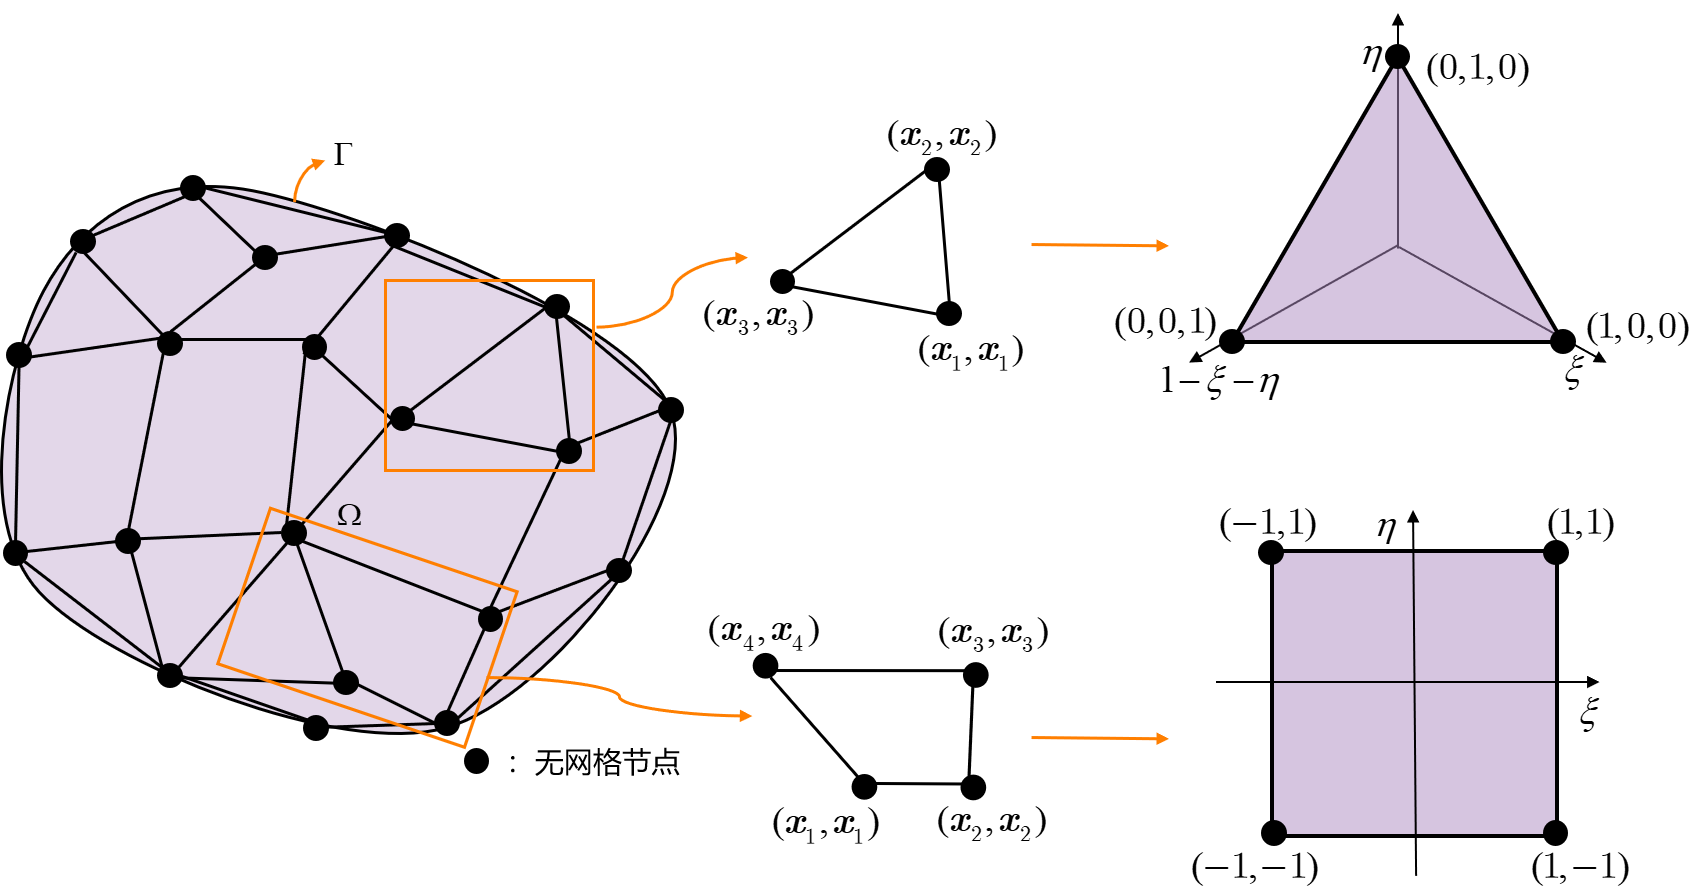
\includegraphics[scale=0.5]{figure/C2/GI.png}
\caption{高斯积分背景网格示意图}\label{C2GI}
\end{figure}
\subsection{再生光滑梯度积分法}
假设场变量$u(\pmb x)$为任意的$p$阶多项式,则其梯度$u_{,i}(\pmb x)$可以表示为:
\begin{equation}
\begin{split}
    u_{,i}(\pmb x)=\pmb a_i^T\pmb q(\pmb x)
\end{split}
\end{equation}
其中$\pmb a_i$表示为任意系数向量;$\pmb q(\pmb x)$为$(p-1)$阶的单项式基向量,即$\pmb q(\pmb x)=\pmb p^{[p-1]}(\pmb x)$,$\pmb{p}(\pmb{x})$是无网格形函数理论中表示$p$阶的多项式基函数向量,根据文献可以知道$(p-1)$阶积分约束条件为:
\begin{equation}\label{p-1}
\begin{split}
    \int_{\Omega}\pmb \Psi_{I,i}\pmb qd\Omega=\int_{\Gamma}\pmb \Psi_I \pmb qn_id\Gamma-\int_{\Omega}\pmb \Psi_I\pmb q_{,i}d\Omega
\end{split}
\end{equation}
根据式子可以看出,由于$p$次基函数,伽辽金弱形式所采用的数值积分方法只有满足$(p-1)$阶积分约束条件,无网格数值解才能重现对应的多项式精确解。\par
根据再生光滑梯度理论,与再生核无网格形函数类似,无网格形函数$\pmb \Psi_I$的再生光滑梯度$\tilde{\pmb\Psi}_{I,i}$可表示为如下形式:
\begin{equation}\label{tildepsi}
\begin{split}
\tilde{\pmb \Psi}_{I,i}(\pmb x)=\pmb q^T(\pmb x)\pmb c_i(\pmb x_I)\tilde{\varphi}(x)
\end{split}
\end{equation}
其中$\pmb c_i$为待定系数向量;$\tilde{\varphi}(\pmb x)$为核函数,这里取为
\begin{equation}
\begin{split}
    \tilde{\varphi}(\pmb x)=\begin{cases}
        1,&\pmb x\in\Omega_c\\
        0,&\pmb x\notin\Omega_c\end{cases}
\end{split}
\end{equation}
其中:$\Omega_C$为互相不重叠且$\cup^{N\!C}_{C=1}\Omega_C=\Omega$的积分单元;
$N\!C$表示的是积分单元的总个数。图(\ref{C2RKGSI})给出了再生光滑梯度无网格法采用采用的三角形背景积分单元。不失为一般性,这里以三次基函数为例详细阐明
再生光滑梯度构造过程。当采用三次基函数$\pmb p(\pmb x)$时,$\pmb q(\pmb x)$的表达式为:
\begin{equation}\label{qx}
\begin{split}
    \pmb q(\pmb x)=(1,x,y,x^2,y^2,xy)^T\quad\pmb x\in\Omega_C
\end{split}
\end{equation}
将式(\ref{qx})代入到积分约束条件式(\ref{p-1})中,可得到:
\begin{equation}\label{tildegc}
\begin{split}
    \int_{\Omega_C}\pmb \Psi_{I,i}\pmb qd\Omega=\tilde{\pmb g}^C_{iI},I=1,2,\dotsb,N\!P
\end{split}
\end{equation}
\begin{equation}
\begin{split}
     \tilde{\pmb g}^C_{iI}=\int_{\Gamma_C}\pmb \Psi_I\pmb qn_id\Gamma-\int_{\Omega_C}\pmb \Psi_I\pmb q_{,i}d\Omega
    \end{split}
\end{equation}
再用式子(\ref{tildepsi})定义的光滑梯度$\tilde{\pmb \Psi}_{I,i}$替换到式子(\ref{tildegc})中的标准梯度$\pmb \Psi_{I,i}$,可以得到$\pmb c_i=\pmb G^{-1}_C\:\tilde{\pmb g}^C_{iI}$
其中$\pmb G_C$为再生光滑梯度的矩量矩阵,其表达式为:
\begin{equation}\label{GC}
\begin{split}
    \pmb G_C=\int_{\Omega_C}\pmb q\pmb q^Td\Omega
\end{split}
\end{equation}
如图(\ref{C2RKGSI})所示,为了方便数值积分再生光滑梯度积分法将三角形积分域投影至参数空间。在投影后的三角形积分域内采用高斯积分法求解得到$\tilde{\pmb g}_{iI}^C$,具体表达式为:
\begin{equation}\label{tildegciI}
\begin{split}
    \tilde{\pmb{g}}_{iI}^C&=\sum_{C=1}^{N\!C}\sum_{G\!B=\mathbb{A}(\Gamma_C)}\Psi_I(\pmb{x}_{GB})\pmb{q}(\pmb{x}_{GB})\pmb{n}_i\pmb{J}(\pmb{x}_{GB})\omega_{GB}\\
    &-\sum_{C=1}^{N\!C}\sum_{G\!I=\mathbb{A}(\Omega_C)}\Psi_I(x_{GI})q_{,i}(x_{GI})J(x_{GI})\omega_{GI}
\end{split}
\end{equation}
其中$\mathbb{A}$为背景积分单元内部或者边界上的高斯积分点总数量;$\pmb{x}_{GB}$、$\pmb{\omega_{GB}}$表示背景积分单元边界上的高斯积分点位置和相应的权重;
$x_{GI}$、$\omega_{GI}$为背景积分单元内的高斯积分点位置与配套的权重;$\pmb{J}$表示背景积分单元联系物理和参数空间的雅可比矩阵行列式。
值得注意的是式(\ref{GC})中的$\pmb{G}_C$不需要采用数值积分计算可以直接解析得到。\par
根据式(\ref{tildepsi})和式(\ref{tildegciI}),可以得到背景积分域内的再生光滑梯度积分表达式为:
\begin{equation}\label{ftildepsi}
\begin{split}
    \tilde{\Psi}_{I,i}(\pmb{x})=\pmb{q}^T(\pmb{x})\pmb{G}^{-1}_C\tilde{g}^C_{iI},\~x\in\Omega_C
\end{split}
\end{equation}
根据式(\ref{ftildepsi})可以看出再生光滑梯度通过直接构造得到,避免了标准无网格梯度的复杂计算,有效的提高了计算精度和计算效率。值得注意的是,再生光滑梯度仅用于刚度矩阵的构造,
对于弹性力学问题中的应力和应变计算,仍然采用传统的无网格形函数及梯度的构造。这是由于再生光滑梯度并非全域连续函数,是在局部背景积分域内满足积分约束条件进而在全域上满足积分约束条件。
\begin{figure}[H]
\centering
    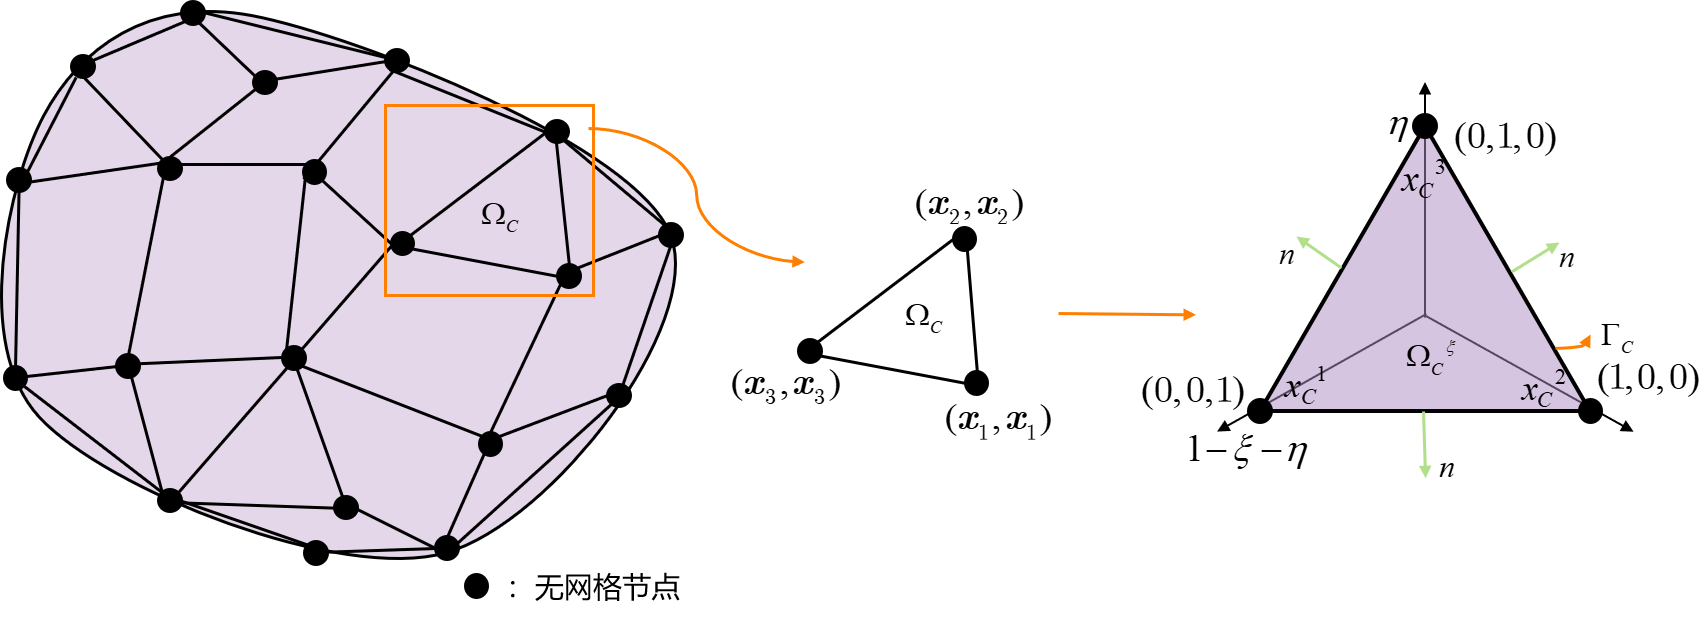
\includegraphics[scale=0.5]{figure/C2/RKGSI.png}
    \caption{三角形背景积分单元示意图}\label{C2RKGSI}
\end{figure}
